\documentclass[border=6pt]{standalone}
\usepackage{tikz}
\usetikzlibrary{positioning}

% Colours approximating the original figure
\definecolor{dirfill}{RGB}{245,230,150}    % goldenrod / khaki (directories)
\definecolor{filefill}{RGB}{210,222,245}   % light blue (files)
\definecolor{nodeline}{RGB}{40,40,120}     % navy
\definecolor{numcol}{RGB}{200,40,40}       % red postorder numbers

\begin{document}
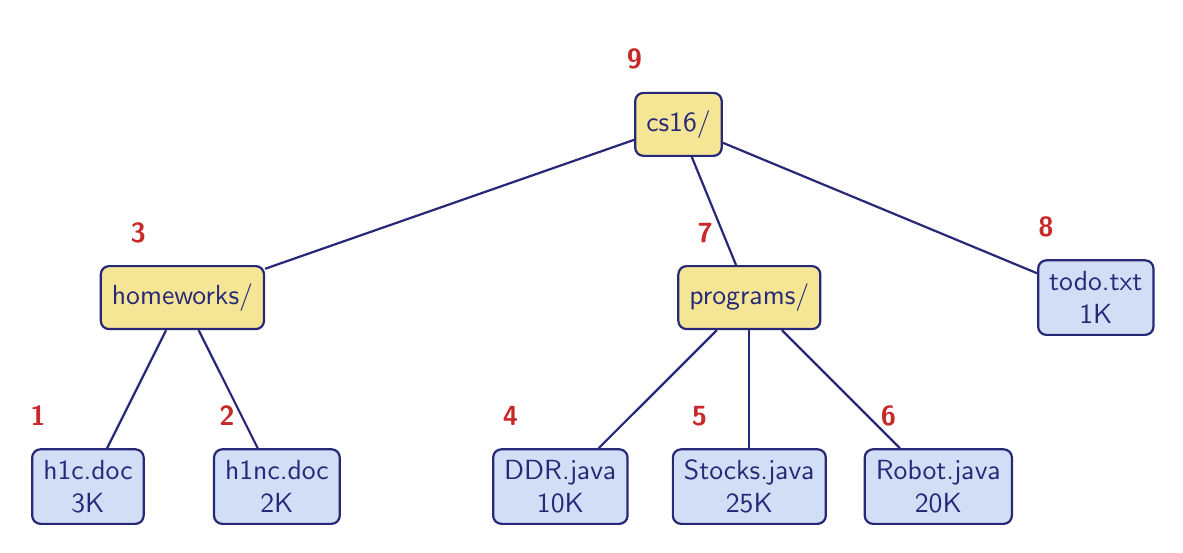
\begin{tikzpicture}[
  font=\sffamily,
  every node/.style={
    draw=nodeline, line width=0.8pt, rounded corners=3pt,
    text=nodeline, align=center, inner sep=4pt, minimum height=8mm
  },
  dir/.style={fill=dirfill},
  file/.style={fill=filefill},
  num/.style={
    draw=none, fill=none, text=numcol, font=\sffamily\bfseries,
    inner sep=1pt
  },
  edge/.style={draw=nodeline, line width=0.8pt},
]

% ---- Nodes (preorder/postorder number given as an above-left label) ----
\node (root)   at ( 1.5, 0)   [dir,  label={[num]above left:9}] {cs16/};

\node (hw)     at (-4.8,-2.2)  [dir,  label={[num]above left:3}] {homeworks/};
\node (prog)   at ( 2.4,-2.2)  [dir,  label={[num]above left:7}] {programs/};
\node (todo)   at ( 6.8,-2.2)  [file, label={[num]above left:8}] {todo.txt\\1K};

\node (h1c)    at (-6.0,-4.6)  [file, label={[num]above left:1}] {h1c.doc\\3K};
\node (h1nc)   at (-3.6,-4.6)  [file, label={[num]above left:2}] {h1nc.doc\\2K};

\node (ddr)    at ( 0.0,-4.6)  [file, label={[num]above left:4}] {DDR.java\\10K};
\node (stocks) at ( 2.4,-4.6)  [file, label={[num]above left:5}] {Stocks.java\\25K};
\node (robot)  at ( 4.8,-4.6)  [file, label={[num]above left:6}] {Robot.java\\20K};

% ---- Edges ----
\foreach \p/\c in {root/hw, root/prog, root/todo,
                   hw/h1c, hw/h1nc,
                   prog/ddr, prog/stocks, prog/robot}
  \draw[edge] (\p) -- (\c);

\end{tikzpicture}
\end{document}
